\chapter{Model referencyjny}

Ze względu na złożoność procesu tworzenia modelu agentowego rynku od podstaw, zdecydowaliśmy się wesprzeć istniejącym modelem agentowym rynku opartego na arkuszu zleceń - ABIDES-em (\textit[Agent-Based Discrete Event Simulator}\cite{abides}). Użycie modelu referencyjnego ma na celu przede wszystkim ominięcie żmudnego procesu kalibracji (dopasowania konfiguracji do prawdziwych danych rynkowych w celu możliwie najlepszego odtworzenia rzeczywistości). Zakładamy, że konfiguracja referencyjna przedłożona przez autorów modelu referencyjnego dobrze odwzorowuje rzeczywistość i koncentrujemy się na rozszerzeniu istniejącego modelu pod kątem modelowania przewagi informacji, przypadku nieuwzględnionego w pierwotnej wersji. 

% sprawdzić dokładnie ABIDESA
Wybrany przez nas framework - ABIDES z założenia miał być narzędziem udostępnionym publicznie na zasadzie \textit{open-source} i służyć do rozwoju projektowania agentów. Od czasu publikacji został wielokrotnie wykorzystany w publikacjach autorów, m.in. do uczenia agentów przy pomocy metod reinforcement learning \cite{abides_reinforcement} czy weryfikowania hipotez na temat wpływu strategii arbitrażowych na zmienność ceny \cite{abides_arbitrage}.

W tej pracy decydujemy się na rozszerzenie modelu w kierunku testowania hipotez związanych z istnieniem przewagi informacyjnej wśród graczy. Zanim jednak przejdziemy do opisu wprowadzonego rozszerzenia i wyjściowych hipotez, nakreślimy działanie modelu referencyjnego. W pierwszej kolejności przyjrzymy się, jakie rozwiązania techniczne zostały zastosowane oraz w jaki sposób przytoczona wcześniej teoria dotycząca projektowania agentów znalazła odzwierciedlenie w implementacji. Następnie opiszemy zaproponowaną przez autorów konfigurację referencyjną, która posłuży nam za bazowy model rynku.

\section{Rozwiązania techniczne} 
\subsection{Chronologia zdarzeń}
W poprzednich rozdziałach skupiliśmy się głównie na elementach modelu specyficznych dla jego zastosowania do modelowania rynku, w domyśle przyjmując, że w symulacji przy pomocy modelu zagwarantowana jest poprawna chronologia zdarzeń. 

W kontekście chronologii zdarzeń warto podkreślić istnienie dwóch odrębnych grup symulatorów: działających w czasie rzeczywistym oraz nie działających w czasie rzeczywistym. Obie grupy cechują inne trudności w zachowaniu prawidłowej chronologii zdarzeń inicjowanych przez agentów. W kontekście modeli agentowych rynku najczęściej implementuje się je przy pomocy symulatorów nie działających w czasie rzeczywistym - w większości przypadków współczesnych zastosowań modeli agentowych motywacją jest sprawdzenie strategii inwestycyjnych lub hipotez na temat hipotetycznych zdarzeń, zatem dążymy do uzyskania możliwie największej próby symulacji. 

Wybrany model referencyjny ABIDES został zbudowany na bazie konceptu \textit{Discrete Event-Based Kernel}\cite{handbook_of_simulation}. W tej metodzie symulacja przebiega w dyskretnych krokach, a centrum symulacji stanowi jądro symulacji pośredniczące w każdym wydarzeniu zachodzącym w trakcie trwania symulacji. Jądro utrzymuje kolejkę priorytetową wszystkich wiadomości wysyłanych przez agentów (czyli, zgodnie z założeniami sekcji \ref{sec:language}, wszystkich wydarzeń zachodzących w symulacji) z kluczem czasu rosnąco. W każdym kroku ustala obowiązujący czas na podstawie najświeższej możliwej wiadomości $m$ i wywołuje metody odpowiedzialne za wykonanie akcji, którą $m$ utożsamia. 
\ref{fig:kerneluml}
\begin{center}
\begin{figure}
\begin{center}
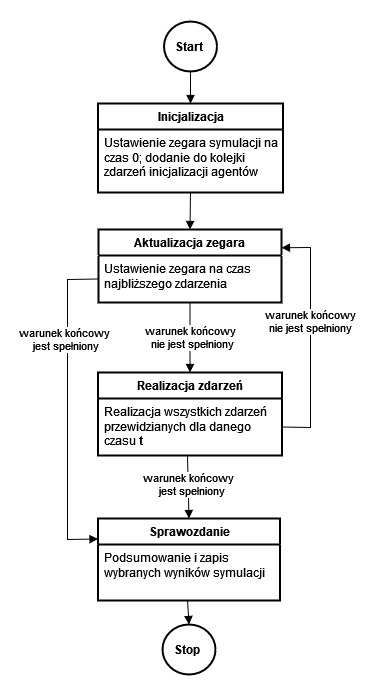
\includegraphics[scale=0.75]{kernel_uml.jpg}
\end{center}
\caption{Ogólny schemat przebiegu pojedynczej symulacji w metodzie \textit{Discrete Event-Based Kernel}, rysunek odwzorowany z \cite{handbook_of_simulation}}\label{fig:kerneluml}
\end{figure}
\end{center}

\subsection{Wyrocznia}

Autorzy ABIDES-a przyjmują założenie, że za zmianę wartości fundamentalnej odpowiada proces stochastyczny typu \textit{mean-reverting}. W dyskretnym wariancie jest on zdefiniowany przez poniższy wzór rekurencyjny \cite{wahwellman}: 
$$r_t = \max\{0,\kappa \bar{r} + (1+\kappa) r_{t-1} + u_t\}; r_0 = \bar{r}, $$
gdzie:
\begin{itemize}
\item $\bar{r}$ - średnia wartość fundamentalna,
\item $\kappa \n [0,1]$ - średni współczynnik powracania,
\item $u_t \sim N(0,\sigma_s)$ - błąd losowy.
\end{itemize}

Procesy typu \textit{mean reversion} dobrze odzwierciedlają cenę w krótkim zakresie czasu \cite{meanreversion} - zakładamy, że, póki nie dojdzie do istotnego w kontekście spółki wydarzenia ekonomicznego, cena stale oscyluje wokół średniej (uczciwej) wartości $\bar{r}$.

Opisany powyżej proces dyskretny ma poważną wadę w kontekście symulacji - jest relatywnie kosztowny obliczeniowo. Obliczenie $r_k$ wymaga obliczenia również $k-1$ poprzednich wartości. Jeśli weźmiemy pod uwagę, że domyślną jednostką symulacji w ABIDES-ie jest nanosekunda, często pojedyncza symulacja będzie wymagała obliczenia $8,64 \times 10^{13}$ kroków, bez względu na złożoność modelu agentowego - wystarczy by jeden z agentów zdecydował się skorzystać z informacji wyroczni w jednym z ostatnich kroków symulacji. Z tego względu w symulatorze zostaje wykorzystany proces stochastyczny ciągły proces Ornsteina-Uhlenbecka \cite{ouprocess}, który możemy traktować jako uogólnienie procesu typu \textit{mean reversion}. 
\subsection{Wielkość zleceń}
W modelu referencyjnym zakładamy istnienie pośród graczy kilku frakcji inwestorów, przy czym każdą frakcję cechuje inny rozkład wielkości zlecenia. Innymi słowy, przyjmujemy założenie, że rozmiar zlecenia składanego przez gracza $\omega$ jest zmienną losową o rozkładzie zdefiniowanym przez mieszankę rozkładów: w pierwszej kolejności przydzielamy graczowi grupę według zamożności zgodnie z prawdopodobieństwami przynależności do jednej z $m$  frakcji $\pi=\{\pi_1,...,\pi_f\},\sum_{i \in [f]} \pi_i =1$, w drugiej kolejności losujemy rozmiar złożonego zlecenia z rozkładu właściwego grupie $f_i$ (tabela \ref{tab:distmix}).

\begin{table}
\caption{Frakcje graczy i ich rozkłady zleceń} 
\label{tab:distmix}
% opisać modify, replace, partial cancel, złożenie 
\begin{center}
\begin{tabular}{ |p{2cm}|p{10cm}|}
\hline
\textbf{$\pi_i$} & \textbf{$f_i$} \\
\hline 0,2 & rozkład logarytmicznie normalny $\mathrm{Lognormal}(\mu=2.9, \sigma^2=1.2)$\\
\hline
 0,7 & rozkład normalny $N(\mu=100, \sigma^2=0.15)$\\
 \hline
 0,06& rozkład normalny $N(\mu=200, \sigma^2=0.15)$\\
 \hline
0,004& rozkład normalny $N(\mu=300, \sigma^2=0.15)$\\
\hline
0,0329 & rozkład normalny $N(\mu=400, \sigma^2=0.15)$\\
\hline
0,001 & rozkład normalny $N(\mu=500, \sigma^2=0.15)$\\
\hline
0,0006 &rozkład normalny $N(\mu=600, \sigma^2=0.15)$\\
\hline
0,0004 &rozkład normalny $N(\mu=700, \sigma^2=0.15)$\\
\hline
0,0005 &rozkład normalny $N(\mu=800, \sigma^2=0.15)$\\
\hline
0,0003 &rozkład normalny $N(\mu=900, \sigma^2=0.15)$\\
\hline
0,0003 & rozkład normalny $N(\mu=1000, \sigma^2=0.15)$\\
\hline
\end{tabular} 
\end{center}
\end{table}
% dać tabelę [prob frakcji][rozkład]
% ewentualnie dopisać tu jakiesś zdanie
\subsection{Implementacja}
Implementacja nie odwzorowuje bezpośrednio teoretycznego podziału na $I$ - instytucję i $E$ - środowisko wprowadzonego w rozdziale 2. (sekcja \ref{sec:theoreticalmodel}), obiekty współtworzące model w swoich atrybutach i metodach mieszają elementy obu teoretycznych warstw. 

Model referencyjny ABIDES został napisany obiektowo. Typy agentów są zdefiniowane w postaci klas. Hierarchię klas agentów w modelu obrazuje schemat \ref{fig:classdiagram}. 
\begin{center}
\begin{figure}
\begin{center}
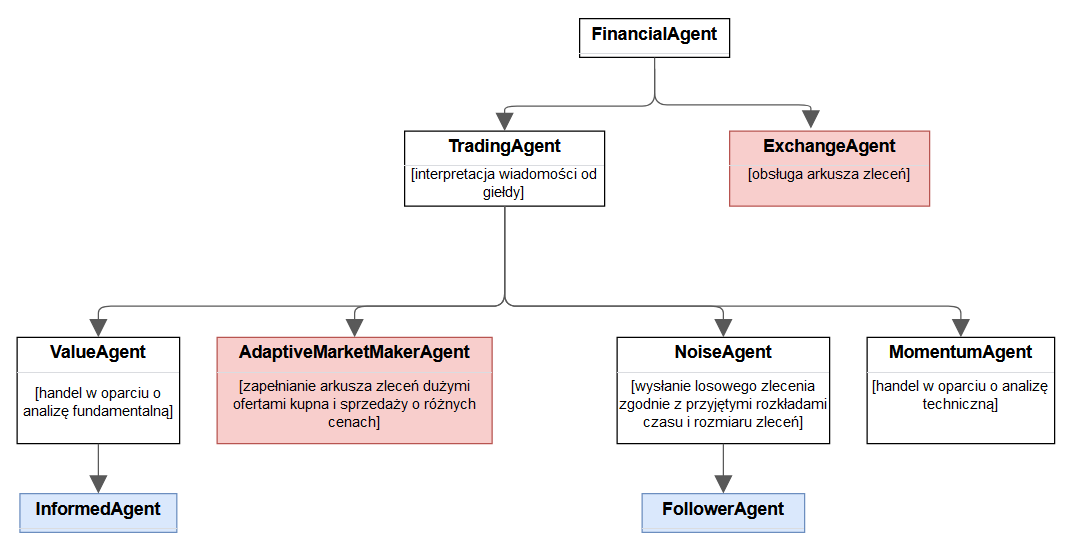
\includegraphics[scale=0.7]{schemat_klas_2.png}
\end{center}
\caption{Schemat klas w modelu i ich podstawowe funkcjonalności. Kolorem czerwonym oznaczeni zostali agenci specjalni (nie modyfikujący strategii), kolorem niebieskim oznaczeni zostali nowo wprowadzeni agenci.}\label{fig:classdiagram}
\end{figure}
\end{center}
Nie będziemy omawiać większości metod i atrybutów klas. Skoncentrujemy się na dwóch kluczowych metodach, które zawierają w sobie całość strategii wybranego typu agenta:
\begin{itemize}
\item \textit{onWakeup} - odpowiada funkcji determinującej aktywność $i.$ gracza $g^i(t_0,t,T)$; określa działania podejmowane przez agenta w momencie obudzenia,
\item \textit{onReceive} - łączy w sobie funkcje alokacji $h^i(m)$ i kosztu $c^i(m)$; określa reakcje agenta na otrzymywane wiadomości, w szczególności aktualizuje stan środków agenta po otrzymaniu potwierdzenia realizacji zlecenia.
\end{itemize}


\section{Konfiguracja referencyjna}

W kontekście celów postawionych w tej pracy najbardziej użytecznym elementem modelu referencyjnego jest załączona do niego konfiguracja referencyjna RMSC04. Kalibracja modelu agentowego, czyli dostosowanie jego parametryzacji w taki sposób, by możliwie najwierniej odzwierciedlał rzeczywistą sytuację, jest, sama w sobie, trudnym i czasochłonnym procesem. Spośród problemów z jakimi należy się zmierzyć w trakcie kalibracji modelu możemy wymienić sposób mierzenia podobieństwa między rzeczywistą sytuacją a próbą jej odwzorowania w symulacji oraz dobór zbioru konfiguracji spośród których będziemy wybierać optymalną. Z wymienionych przyczyn, trudno byłoby włączyć etap kalibracji modelu w zakres pracy. 

Konfiguracja referencyjna RMSC04 (tabela \ref{tab:refconfig}) jest konfiguracją opracowaną przez jego autorów w momencie rozszerzenia frameworku o tworzenie w oparciu o model agentowy środowisk do uczenia agentów uczonych przez wzmacnianie (reinforcement learning) \cite{abides_gym}. Wzorowana jest na rynkach giełdy amerykańskiej giełdy papierów wartościowych NASDAQ\cite{nasdaq} i zawiera wyłącznie agentów typu Zero Intelligence oraz Zero Intelligence Plus. 

Niestety, w swoich pracach oraz w repozytorium symulatora, autorzy ABIDES-a nie opisali procesu kalibracji modelu czy też uzasadnienia zmian, jakich dokonali względem pierwotnej konfiguracji RMSC03, załączonej do pierwszej wersji symulatora \cite{getreal}. W RMSC04 wprowadzono jedną znaczącą zmianę względem RMSC03 - wykluczono z niej agentów typu Heuristic Belief Learning, przypuszczalnie głównie z powodów wydajnościowych (przyp. agenci typu HBL wymagają pobierania danych o wszystkich zleceniach z ustalonego okresu $T$ w każdym kroku). 

\begin{table}
\caption{Skład konfiguracji referencyjnej RMSC04}\label{tab:refconfig}
\begin{center}
\begin{tabular}{|p{3cm}|p{3cm}|p{4cm}|p{3cm}|}
\hline
\textbf{klasa agenta} & \textbf{typ agenta} & \textbf{model obudzeń} & \textbf{liczba agentów}\\
\hline
ExchangeAgent & - & - & 1\\
\hline
AdaptiveMarketMakerAgent & Zero Intelligence Plus & narzucona częstotliwość: 60s &1\\
\hline
ValueAgent & Zero Intelligence Plus & proces Poissona z $\lambda=5.7^{-12}$ & 102\\
\hline
MomentumAgent & Zero Intelligence Plus & narzucona częstotliwość: 60s & 12 \\
\hline
NoiseAgent & Zero Intelligence & zgodnie z rozkładem U-kwadratowym&1000\\
\hline
\end{tabular} 
\end{center}
\end{table}

Wybrana konfiguracja referencyjna zawiera agentów pięciu różnych typów (klas), z czego dwóch specjalnych (oznaczonych również na schemacie \ref{fig:classdiagram}): \textit{ExchangeAgent} oraz \textit{AdaptiveMarketMakerAgent}. ExchangeAgent to agent - giełda, którego jedynym zadaniem jest obsługa rynku (arkusza zleceń) i nie uczestniczy w transakcjach kupna lub sprzedaży jako strona. Z kolei AdaptiveMarketMakerAgent to agent reprezentujący animatora rynku (ang. \textit{market makera}), czyli współpracujący z giełdą podmiot mający zapewnić ciągłość handlu na giełdzie poprzez zobowiązanie do składania regularnie równocześnie ofert kupna i sprzedaży spełniających umówione kryteria pod względem m.in. cen i wielkości ofert. Animator rynku, poza zyskiem z handlu instrumentem, może również otrzymywać wynagrodzenie ze strony giełdy lub emitenta papierów wartościowych, czego model agentowy rynku nie uwzględnia. Obaj gracze realizują ustalone akcje, których nadrzędnym celem jest płynne działanie rynku, ich sposób działania nie podlega modyfikacji. Używając terminu \textit{gracze} o agentach modelu, będziemy domyślnie pomijać agentów wspomnianych klas.

Pozostałe trzy klasy agentów uwzględnione w konfiguracji referencyjnej to typy agentów podobne do występujących już wcześniej w literaturze. \textit{NoiseAgent} to minimalnie zmodyfikowany klasyczny agent Zero Intelligence, wysyłający losowe zlecenia. Natomiast klasy \textit{ValueAgent} i \textit{MomentumAgent} nawiązują do podziału na agentów podejmujących decyzje w oparciu o analizę techniczną oraz agentów podejmujących decyzję w oparciu o analizę fundamentalną, opisanego szerzej w sekcji \ref{sec:ziplus}
